%%%% This CV has been greatly influence by
%%%% the extended fancy cv from Carmine Benedetto.
%%%% I thank him for the excellent work. Unfortunately 
%%%% it wouldn't compile on my machine. So I worked it out myself.

\documentclass{article} 
\usepackage[ngerman]{babel}% deutsche Trennregeln
\usepackage{microtype}% verbesserter Randausgleich
\usepackage[utf8]{inputenc}
\usepackage{graphicx}
\usepackage{color}
\usepackage{xcolor}
\usepackage[obeyspaces]{url} 
\usepackage[left=0.5cm,top=0.25cm,right=1.5cm,bottom=0.5cm,nohead,nofoot]{geometry}

\usepackage{fontawesome}


\makeatletter
\setlength{\@fptop}{40pt}
\makeatother

\usepackage{pdfcomment}
% Fix incorrect display of tooltips (http://tex.stackexchange.com/a/74340/3323)
\makeatletter
\renewcommand{\pc@annot@tooltip}%
{%
  /TU (\pc@pdfenc@contents)\space%
  /T (tooltip \thezref@unique)\space%
  /C [0 0 0]\space%
  /FT/Btn\space%
  /Ff 65536\space%
  /H/N\space%
}%

  
\definecolor{white}{RGB}{255,255,255}
\definecolor{anti-flashwhite}{rgb}{0.95, 0.95, 0.96}

\definecolor{darkgray}{HTML}{333333}
\definecolor{gray}{HTML}{4D4D4D}
\definecolor{lightgray}{HTML}{999999}

\definecolor{green}{HTML}{C2E15F}
\definecolor{orange}{HTML}{FDA333}
\definecolor{purple}{HTML}{D3A4F9}
\definecolor{red}{HTML}{FB4485}
\definecolor{blue}{HTML}{6CE0F1}
\definecolor{pblue}{HTML}{0395DE}

\usepackage[framemethod=tikz]{mdframed}
\usepackage{tikz}
\newcommand*{\ClipSep}{0.4cm}%


\usepackage{hyperref}
\hypersetup{
    pdftitle={},
    pdfauthor={},
    pdfsubject={},
    pdfkeywords={},
    colorlinks=false,       % no lik border color
   allbordercolors=white    % white border color for all
}
 
\pagestyle{empty}

\begin{document}
\begin{mdframed}[backgroundcolor=anti-flashwhite]
	\begin{minipage}[t]{0.4\textwidth}
	{\fontsize{30pt}{62pt}\color{gray} \selectfont {Silvio}{\textbf{Schwarz}}}\\
    {\fontsize{14pt}{24pt}\color{pblue} \selectfont Geophysicist \color{lightgray} (B.Sc.)}\\\\\\
    \textbf{\underline{Philosophy}}:
    \begin{itemize}
    \item open-source, transparent
    \item failure is part of progress
    \item reliability beats sophistication
    \end{itemize}
	\end{minipage}
	\hfill
	\vrule
	\hfill
	\begin{minipage}[t]{0.2\textwidth}
	\vspace{0cm}
	\begin{tikzpicture}
\node [inner sep=0pt] at (0,0) {
\includegraphics[trim=0cm 12cm 0cm 0cm, clip,scale = 0.1]{img/ich2.jpg}};
\draw [anti-flashwhite, rounded corners=\ClipSep, line width=\ClipSep] 
    (current bounding box.north west) -- 
    (current bounding box.north east) --
    (current bounding box.south east) --
    (current bounding box.south west) -- cycle
    ;
\end{tikzpicture}
	\end{minipage}
	\hfill
	\begin{minipage}[t]{0.25\textwidth}
	\vspace{0.25cm}
	{\color{pblue}Address}\\
	Zeppelinstraße 162, 3.2\\
	14471 Potsdam. Germany
	
	\vspace{0.15cm}
	{\color{pblue}Telephone}\\
	01746507598
	
	\vspace{0.15cm}
	{\color{pblue}Email}\\
	\href{mailto:silvio\_ schwarz@web.de}{silvio{\_}schwarz@web.de}
	
	\vspace{0.15cm}
	{\color{pblue}Web}
	
	\vspace{0.15cm}
	{\Large \href{https://github.com/silvioschwarz}{\faGithub}  \hfill \href{silvioschwarz.}{\faSkype} \hfill \href{https://www.linkedin.com/in/silvioschwarz/}{\faLinkedin} \hfill \href{https://silvioschwarz.github.io}{\faGithubAlt}}
	\end{minipage}
\end{mdframed}
\vspace{0.015cm}
\begin{minipage}[t]{0.3\textwidth}
	\centering
	\section*{\hfill \fontsize{18pt}{24pt}\selectfont \color{pblue} Global Experience}
	\vspace{-2mm}
	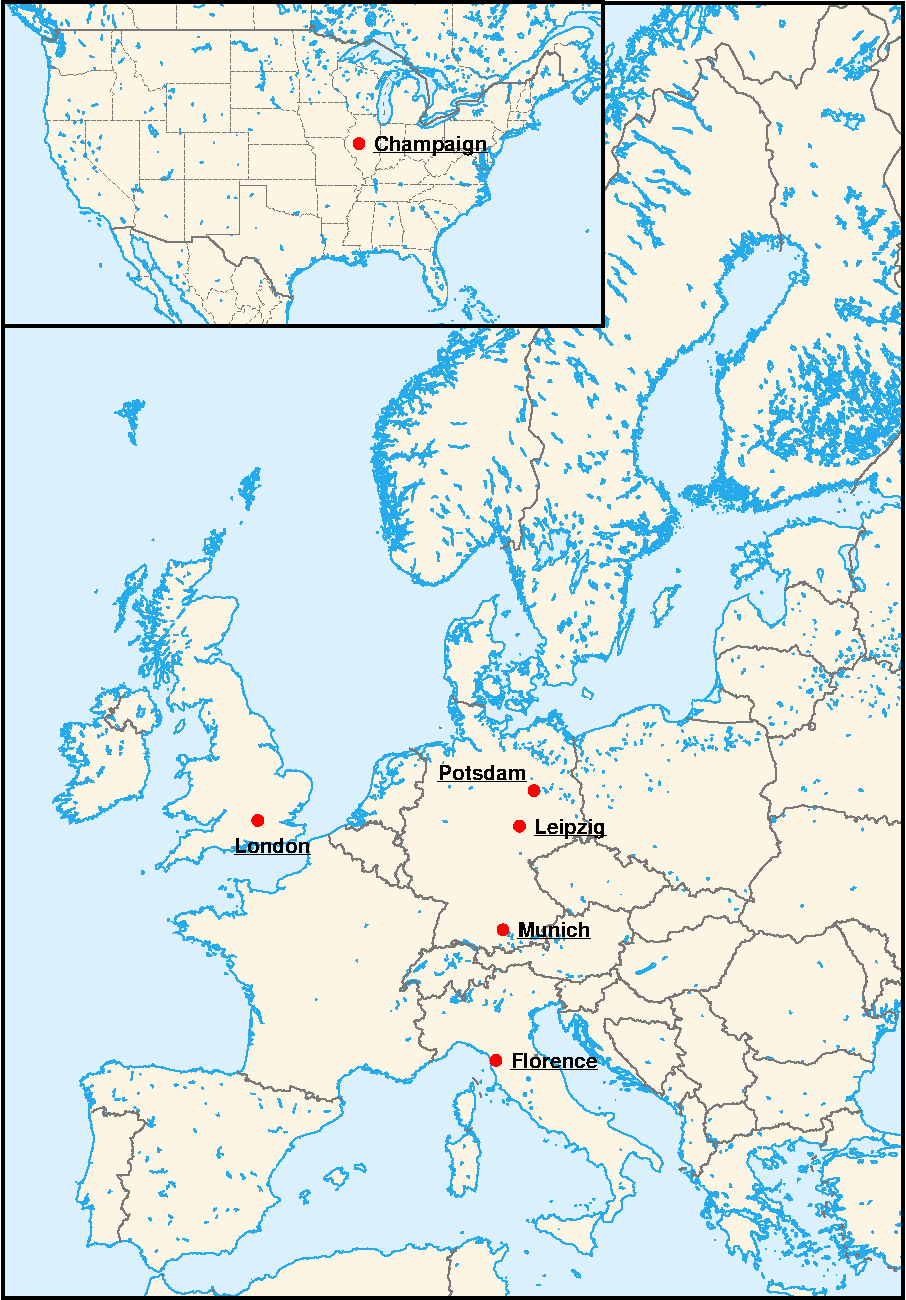
\includegraphics[scale=0.3]{img/globalEXPeng.pdf}
	\vspace{2mm}
	\hrule
	\vspace{-3mm}
	\section*{\fontsize{18pt}{24pt}\selectfont \color{pblue} OS Preference}
	\vspace{-2mm}
	\begin{itemize}
	\centering
	\item[\textbf{\LARGE \faLinux}]
\includegraphics[scale=0.50]{img/5stars.png}\vspace{-2mm}
	\item[\textbf{\LARGE \faWindows}]
\includegraphics[scale=0.50]{img/4stars.png}\vspace{-2mm}
    \item[\textbf{\LARGE \faApple}]
\includegraphics[scale=0.50]{img/1stars.png}
    \end{itemize}
	\hrule
	\vspace{-2mm}
    \section*{\fontsize{18pt}{24pt}\selectfont \color{pblue} Programming}
	\vspace{-2mm}
	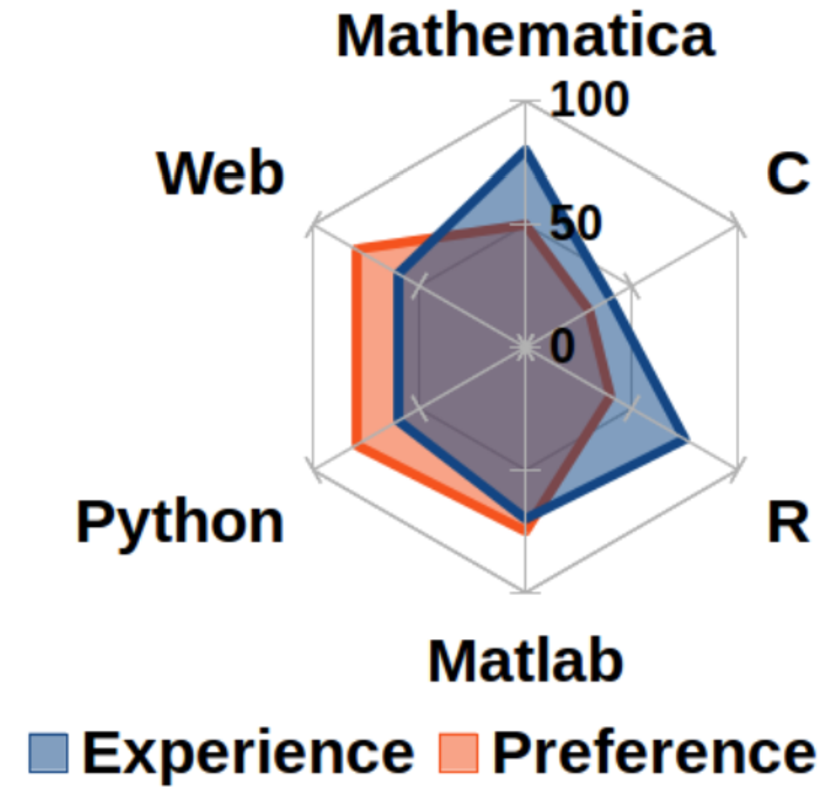
\includegraphics[scale=0.3]{img/programming.pdf}
	\vspace{2mm}
	\hrule
	\vspace{-2mm}
	\section*{\fontsize{18pt}{24pt}\selectfont \color{pblue} Languages}
	\vspace{-2mm}
	\begin{itemize}
	\centering
	\item[\textbf{German}] 
\includegraphics[scale=0.50]{img/5stars.png}\vspace{-2mm}
	\item[\textbf{English}]  
\includegraphics[scale=0.50]{img/4stars.png}\vspace{-2mm}
    \item[\textbf{Italian}] 
\includegraphics[scale=0.5]{img/3stars.png}\vspace{-2mm}
    \item[\textbf{French}]  
\includegraphics[scale=0.50]{img/2stars.png}
    \end{itemize}
	\hrule
	\vspace{-2mm}
	 \section*{\fontsize{18pt}{24pt}\selectfont \color{pblue} Interests}
	\vspace{-2mm}
	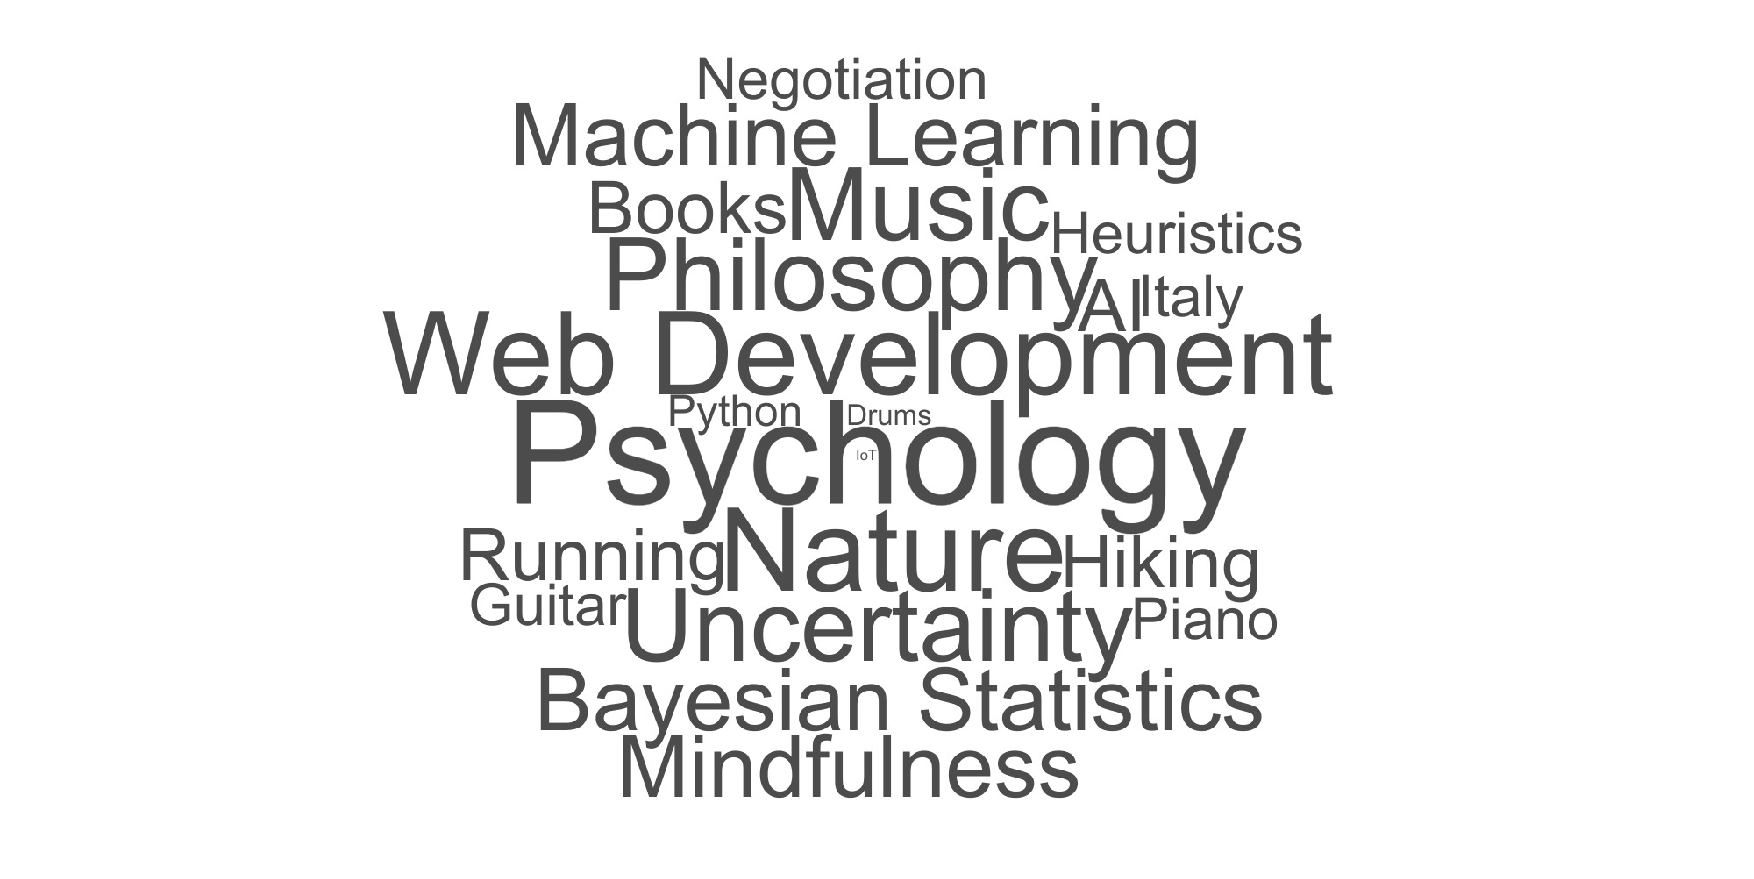
\includegraphics[trim=6cm 1cm 6cm 1cm, clip,scale=0.25]{img/wordcloud2.pdf}
\end{minipage}
\vrule
\hfill
\begin{minipage}[t]{0.65\textwidth}
		\section*{\fontsize{18pt}{24pt}\selectfont \color{pblue} Education}
		\begin{minipage}{0.31\textwidth}
	\textbf{\color{pblue}\faHourglassHalf~Master of Science} \\
	\textbf{Earth Sciences}\\
	\textbf{\underline{Focus:}~Geophysics}\\\\
	\textbf{\underline{Thesis}}:\\\\\\\\\\\\
		10/2011 - present\footnote{longer break due to illness}\\
	Universität Potsdam
		\end{minipage}
		\hfill
		\begin{minipage}{0.33\textwidth}
	\textbf{\href{https://www.dropbox.com/s/297g1chiby8mrd3/Bachelor-Certificate.pdf?dl=0}{\color{pblue}\faGraduationCap~Bachelor of Science}}\\
	\textbf{Earth Sciences}\\\\\\
	\textbf{\underline{Thesis}}:\\
	\href{https://www.dropbox.com/s/3kngo4hpb0c47ww/Bachelorarbeit.pdf?dl=0}{\pdftooltip{Simulation von Bodenbewegungsszenarien von Starkbeben (German)}{engl.: Simulating Ground Motion Scenarios of strong Earthquakes}}\\\\\\
	{10/2008 - 09/2011}\\
Universität Potsdam\\\\
		\end{minipage}
		\hfill
		\begin{minipage}{0.3\textwidth}
	\textbf{\href{https://www.dropbox.com/s/nsgmvy7o64xb9si/Abiturzeugnis.pdf?dl=0}{\color{pblue}\faGraduationCap~Abitur}}\\
	\textbf{Math}\\
	\textbf{Geography}\\\\
	\textbf{\underline{Thesis}}:\\
	 \pdftooltip{Naturkatastrophen und ihr Einfluss auf das Leben in der Gegenwart (German)}{engl.: Natural Disasters and their Impact on Life in the Present}\\\\
	 08/2000 - 05/2008\\
Klosterschule Roßleben (staatl. Gymnasium)\\
		\end{minipage}
		\hrule
		\section*{\fontsize{18pt}{24pt}\selectfont \color{pblue} Work Experience}		
		\begin{minipage}[t]{0.3\textwidth}
		08/2014 - 06/2015\\ (11 Monate)
		\end{minipage}
		\hfill
		\begin{minipage}[t]{0.7\textwidth}
		\textbf{Werksstudent}\hfill \href{https://assecor.de/}{\color{pblue}Assecor GmbH}\\
	    Support in documentation of the power grid ofBerlin, Germany for Vattenfall Europe Sales GmbH
		\end{minipage}\vspace{0.5cm}
		
		\begin{minipage}[t]{0.3\textwidth}
		11/2013 - 03/2014 \\ (5 Monate)
		\end{minipage}
		\hfill
		\begin{minipage}[t]{0.7\textwidth}
		\textbf{Werksstudent}\hfill \href{https://assecor.de/}{\color{pblue}Assecor GmbH}\\
	    Migration of the IT Infrastructure to Windows 7 for\\ BIOTRONIK SE \& Co. KG
		\end{minipage}\vspace{0.5cm}

		\begin{minipage}[t]{0.3\textwidth}
		09/2012 - 11/2012 \\ (3 Monate)
		\end{minipage}		
		\hfill
		\begin{minipage}[t]{0.7\textwidth}
		\textbf{Praktikum}\hfill \href{https:///www.wolframalpha.com/}{\color{pblue}Wolfram$\mid$Alpha, IL, USA}\\
	    Research and Development\\
	    Development of geophysical content for Wolfram$\mid$Alpha
		\end{minipage}\vspace{0.5cm}
		
		\begin{minipage}[t]{0.3\textwidth}
		06/2011 - 08/2012 \\ (1 Jahr 3 Monate)
		\end{minipage}
		\hfill
		\begin{minipage}[t]{0.7\textwidth}
		\textbf{studentischer Assistent}\hfill \href{https://www.uni-potsdam.de/}{\color{pblue}Universität Potsdam}\\
	    Geophysical prospection, seismological model building and consult for the Council for Geoscience, Pretoria, South Africa
		\end{minipage}\vspace{0.5cm}
		
		\begin{minipage}[t]{0.3\textwidth}
		03/2010 - 05/2010 \\ (3 Monate)
		\end{minipage}
		\hfill
		\begin{minipage}[t]{0.7\textwidth}
		\textbf{studentischer Assistent}\hfill \href{https://www.uni-potsdam.de/}{\color{pblue}Universität Potsdam}\\
	    Quality control of algorithms used in the scope of seismic hazard analysis
		\end{minipage}
\end{minipage}
\end{document}